\chapter*{О кирпичной глине}
\addcontentsline{toc}{chapter}{О кирпичной глине}

\textbf{Из «Статистическое описание Киевской губернии», часть 1, издание Фундуклея (1852)}:\\

Кирпичная глина. Она находится в изобилии во всех уездах губернии, особенно в степных, но лучшая из них в г. Киеве и его окрестностях, а также возле Межигорской фабрики в с. Петровцах. В Киеве главные места разработки этой глины находятся в крутом обрыве гор, идущих вдоль низменной улицы, называемой Плоскою. Там выказывается наружу толстый пласт ее, первый снизу; на котором лежат все прочие пласты тех гор. 

Сырые кирпичи из этой глины зеленоватого светлого цвета, но будучи обожжены, принимают светло-красноватый вид. Качеством они очень хороши, особенно для кладки печей, но процент утраты при обжигании довольно значителен. В окрестностях города, особенно за Печерскою частью, кирпич выходит еще доброкачественнее, желтоватого цвета, и употребляется в значительном количестве на крепостные постройки. На некоторых низменных, ровных местах, прилегающих к Днепру, по Оболони, попадается красно-бурая глина, из которой кирпич выходит темнокрасный, и тоже очень доброкачественный. Но Межигорская глина еще лучше Киевских. Из нее приготовляется кирпич беложелтоватого цвета, особенно годный для стен фундаментов, ибо упорен против влияния влажности, обстоятельство немаловажное для Подольской и плоской части г. Киева, часто, затопляемых весной разливом Днепра.

Там же приготовляют еще другой сорт кирпича, малого формата, совершенно белый, уподобляющийся сахарным плиткам и употребляемый на выкладку пода в печах и на самые печи; глина, из которой его делают – весьма огнеупорна. Там же добывают кафельную или изразцовую глину, которую привозят и на Киевские заводы в сыром виде, для обработки.[...]

Горшечная глина находится во многих уездах, и преимущественно в Киевском и в Таращанском, при устье р. Лыбеди в Киеве и в Межигорье; [...] Кроме посуды из нее приготовляют доброкачественные изразцы для печей.[...]

Фаянсовая глина находится целыми слоями в окрестностях г. Киева при устье р. Лыбеди, но еще в значительнейших массах и лучшего качества возле Межигорской фаянсовой фабрики.\\


\textbf{«Химическое исследование киевских глин», С. Богданов, Записки Киевского общества естествоиспытателей, том 7, выпуск 1 (1883):}\\

Киевская синяя (спондилувая, кирпичная) глина\footnote{«Образец для исследования был взят на кирпичном заводе г. Субботина» – прим. С. Богданова).}.

Киевская синяя глина принадлежит второму ярусу киевской третичной эосеновой формации. На площади Киева она залегает на уровне Днепра, образуя подошву поверх лежащих более новых третичных образований.

Во влажном состоянии она имеет темно-зеленый цвет, при высыхании же зеленовато-серый; кирпич из нея приготовленный – светло-желтого цвета. Влажная глина мягка, с слабым блеском; липнет к языку. Ломается синяя глина глыбами, имеющими широко-раковистый землистый излом и плоскость разреза с матовым блеском. В воде отчасти листится и распускается трудно, не производя мути; при этом наблюдается обильное выделение пузырьков воздуха, сопровождающееся характерным шумом (в роде свиста).

Смоченная глина имеет довольно ясный аммиачный запах. При действии кислот сильно шипит вследствие обильного выделения пузырьков углекислоты. Макро и микроскопическое исследование, кроме глинистой части, окрашенной примесью бурого железняка, обнаруживает еще кварцевый песок, блестки сере\-бристо-белой слюды и мелкие зерна главконита. В некоторых образцах синей глины можно также заметить мелкие желваки железного колчедана, мергельные сростки, содержащие фосфорно-известковую соль, и наконец обыкновенно кристаллы гипса. Значительного количества полевого шпата не видно (сообщено К. М. Феофилактовым). При отмучивании уже самые первые порции, состоящие из наиболее мелких частиц, окрашены в зеленоватый цвет и содержат некоторое количество кварцевого песка.

Объем 1 gr. сухой глины, вобравшей в себя возможное количество воды, равен 1,9 c.c.m. (среднее из двух чисел: 1,84 c.c.m. и 1,91 c.c.m.). Водоемкость 1,3 (среднее из двух чисел: 1,24 и 1,30). Maximum гигроскопичности 6,69 (среднее из двух чисел: 6,78 и 6,61). Таким образом синюю глину следует признать весьма пластичною.

При накаливании приготовленного из нея цилиндрика уже при 1000° C. происходит настоящее плавление, следовательно она весьма легкоплавка. С этим выводом вполне гармонирует и ничтожный коэффициент огнеупорности синей глины, равный 0,02.

Употребляется синяя глина на многочисленных киевских кирпичных заводах для изготовления строевого кирпича прекрасных качеств.

Первый полный элементарный анализ ея принадлежит г. Рожанскому\footnote{«Зап. К. О. И. Р. Т. О. 1881, XI, 11» – прим. Богданова.}, важнейшие результаты которого потом подтвердил г. Марциновский\footnote{«Частное сообщение. Аналиы гг. Рожанского и Марциновского были произведены также в Технической лаборатории Университета св. Владимира» – прим. Богданова.}, и вследствие этого отсутствие необходимости повторять их исследование. Таким образом я занялся преимущественно вопросом о ближайших составных частях этой глины. Результаты всех указанных выше элементарных анализов синей глины представляет следующая таблица.


\begin{center}
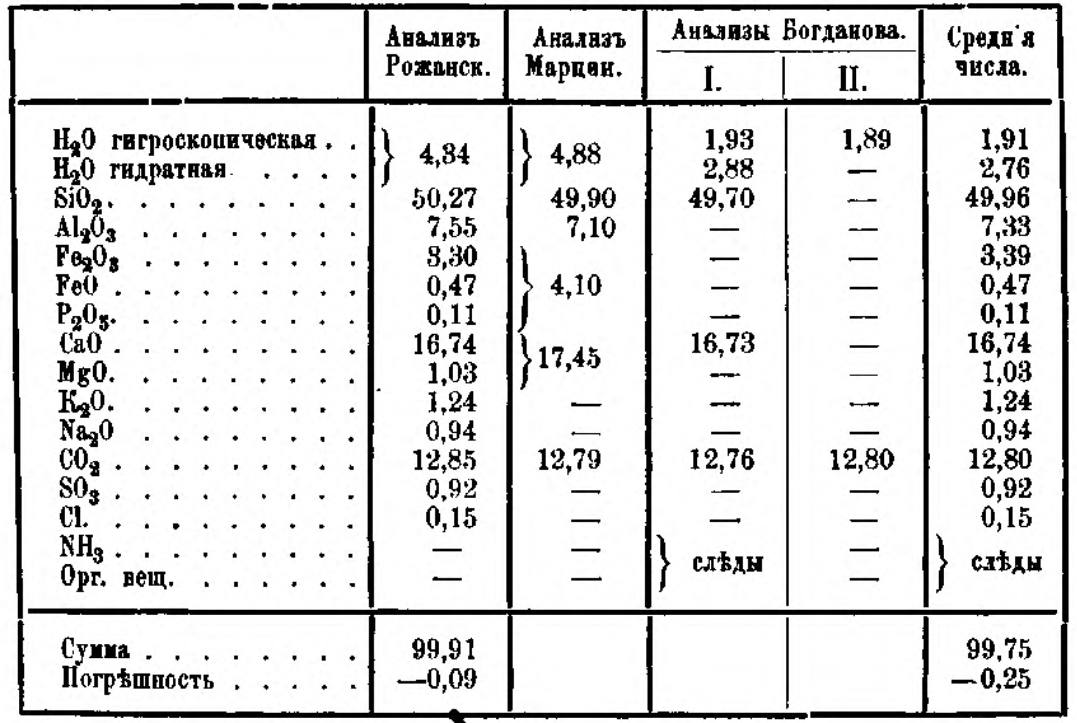
\includegraphics[width=\linewidth]{pix/table-01.jpg}
\end{center} 

В анализах гг. Рожанского и Марциновского не приведены отдельные числа для H$_2$O гигроскопической и гидратной, потому что эти исследователи принимаю за гигроскопическую воду в глинах потерю, претерпеваемую последними выше 120° C., что несогласно с изложенным выше моим взглядом на этот предмет.

Содержание в синей глины разных видов химически соединенной воды по моим определениям, следующее:\\


\begin{tabular}{| l | l |}
\hline
H$_2$O непрочно соед. & 0,96 \\
H$_2$O прочн. соедин. & 1,80 \\
\hline
\end{tabular}\\

(К 1,80 Богданович делает примечание: «Найденная гг. Рожанским (2,86\%) и Марциновским (2,92\%) потеря синей глины при 120° C., равная сумме гигроскопической и непрочно соединенной воды весьма близко подходит к той же сумме, составленной на основании моих определений (0,96\%+1,80\%=2,76\%)»).

Из общего количества SiO$_2$, по определению г. Рожанского, в синей глине заключается\\

\begin{tabular}{| l | l |}
\hline
Кварцевого песка & 32,03\\
SiO$_2$ химич. соедин. & 18,24 \\
\hline
\end{tabular}\\

(К 32,03 Богданович примечает: «Определяется нагреванием глины с серной кислотой в запаянной трубке и т.д., как в пестрой глине».)

При произведенных же мною и г. Марциновским опытах кипячения глины с серной кислотой в платиновой чашке, с последующей обработкой нерастворимого остатка кипящим раствором соды, получилось:\\

\begin{center}
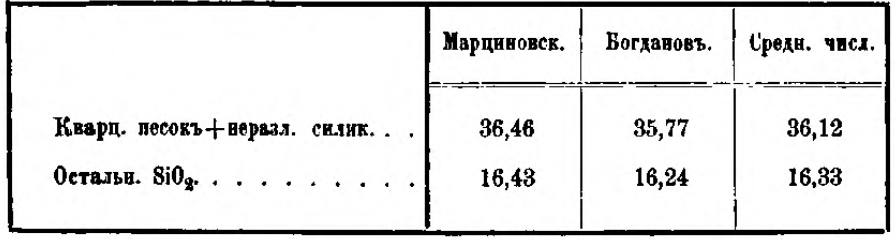
\includegraphics[width=\linewidth]{pix/table-02.jpg}
\end{center} 

Вычитая из суммы кварцевого песка + неразложившийся силикат полученное г. Рожанским число для чистого кварцеватого песка, я нахожу, что силикат, неразлагаемый кипящею серною кислотою при атмосферном давлении, заключается в синей глине в количестве 4,09\%. Если же от суммы кварцеватого песка + неразложившийся силикат + остальной SiO$_2$ (равной 52,45\%) отнять общее содержание SiO$_2$, то окажется, что основания в указанном силикате составляю 2,49\%.

Относительно природы этого соединения можно сделать заключение уже на основании микроскопического исследования синей глины, так как из всех найденных в ней этим способом силикатов лишь поташистая слюда не разлагается серною кислотою при кипячении в открытом сосуде. И микроскопическое исследование нерастворимого остатка, полученного при моем опыте, указывает на присутствие здесь кварца и слюды (сообщение г. Армашевского). Приняв для поташистой слюды типическую формулу K$_2$O. Al$_2$O$_3$. 2SiO$_2$, я, по общему содержанию оснований, нахожу, что K$_2$O в поташистой слюде синей глины составляет 1,18\%, Al$_2$O$_3$ 1,31\%, SiO$_2$ 1,51/%.

Отнимая сумму оснований + вычисленное количество SiO$_2$, слюды от суммы кварцевого песка + неразложившийся силикат, я определяю непрямым способом содержание чистого кварцевого песка в синей глине, которое оказывается равным 32,12\%, – число весьма близкое к найденному г. Рожанским, что указывает на правильность оснований его определения и, вместе с тем, на правильном допущения в нерастворимом в серной кислоте остатке глины только кварца и поташистой слюды.

Взяв средние числа из всех прямых и непрямых определений кварцевого песка в синей глине и приняв остальной SiO$_2$ <ся>  за химически соединенный, нахожу, что здесь содержится\\ 

\begin{tabular}{| l | l |}
\hline
Кварцевого песка & 32,08 \\
SiO$_2$ химич. соедин. & 18,88 \\
\hline
\end{tabular}\\

Среднее же содержание поташистой слюды нужно выразить числом 4,0\%, которое впрочем следует считать только приблизительным, так как определение поташистой слюды основано на допущении совершенной неразлагаемости ея при кипячении с серной кислотой в платиновой чаше, так как она при этом уже несколько разлагается.

При определении прочих ближайших составных частей синей глины гораздо более важное значение, чем для двух предыдущих глин, имеет обработка ея разными реактивами. Так, уже вода извлекает из синей глины довольно значительное количество примесей: следы органических веществ, немного Cl, Na и довольно много CaO и CO$_3$.

На основании этих данных я заключаю о присутствии в синей глине небольших количеств NaCl и органических (вероятно, как и в предыдущих глинах, частью в виде известковых солей перегнойных кислот), а также значительного количества гипса, общее содержание которого определяю на том основании, что после обработки водою в глине уже не оказывается SO$_3$, который следовательно, весь входит в состав гипса. Таким образом в последнем заключается SO$_3$ – 0,92\%, CaO – 0,64\%, 2H$_2$O – 0,41\%, общее же количество гипса равно 1,97\%. Обе частицы воды гипса принадлежат к непрочно соединенной воде глины, так что на прочие составные части синей глины остается воды непрочно связанной всего 0,55\%.

Общее содержание NaCl определяется количеством Cl, заключающегося только в NaCl: Cl – 0,15\%, Na – 0,09 – NaCl составляет таким образом 2,24\%.

Уксусная кислота на холоду выделяет из синей глины CO$_2$, и извлекает в раствор очень много CaO меньше MgO, немного Fe$_2$O$_3$, Al$_2$O$_3$ и SiO$_2$, также весьма мало P$_2$O$_3$. После этой обработки в глине остаются только следы P$_2$O$_3$, которые извлекаются соляной кислотой, так что, принимая во внимание преимущественное распространение в природе из фосфатов, разлагаемых уксусною кислотою – известкового, а из неразлагаемых уксусной кислотой, но поддающихся действию соляной кислоты – фосфата Fe$_2$O$_3$, следует заключить о присутствии в синей глине некоторого количества Ca$_3$(PO$_4$)$_2$ и следов FePO$_4$. Fe$_3$(PO$_4$)$_2$ в исследуемой глине нет, так как уксусно-кислая вытяжка не заключает вовсе FeO. Относя весь P$_2$O$_3$ к Ca$_2$(PO$_4$)$_2$ и пренебрегая ничтожным количеством его в виде FePO$_4$, получаю, что в синей глине Ca$_3$(ЗЩ$_4$)$_2$ составляет 0,26\% (P$_2$O$_5$ – 0,11\%, CaO – 0,15\%).

Принимая во вниманием, что после обработки уксусной кислотой в глине не остается сколько-нибудь значительного количества CaO, я считаю возможным всю остальную CaO, кроме заключающейся в гипсе и Ca$_3$(PO$_4$)$_2$, т.е. 15,59\%, отнести к CaCO$_3$; в таком случае в этой соли заключается CO$_2$ 12,53\%, общее же количество CaCO$_3$ синей глины равно 28,48\%.

Остальная CO$_2$ (2,27\%) соединена с MgO, так что количество MgO$_3$ равно 0,52\%.

Правильность выводов относительно общего содержания в синей глине CaCO$_3$, MgCO$_3$, гипса и Ca$_3$(PO$_4$)$_2$ подтверждается тем, что при обработке глины уксусной кислотой до прекращения вы <далее у меня нет страниц>[...]

Например, киевская синяя глина, содержащая около 4\% бурого железняка, при слабом прокаливании окрашивается в желтый цвет, но при более высоких температурах, когда начинается сплавление глины, она получает черную окраску, что вероятно зависит от главконита, который в чистом состоянии показывает ту же особенность.[...]

Еще меньше коалина в киевской синей глине (около 10\%), главные составные части которой – кварцевый песок (32\%) и CaCO$_3$ (28 1/2\%), так что синюю глину правильнее называть песчаным мергелем. Зеленоватый цвет ея зависит от присутствия около 2\% главконита. Она весьма пластична и легкоплавка.
